\documentclass[12pt,twoside]{extarticle}
\usepackage[margin=1.2in,top=1.6in,bottom=1.6in]{geometry}
\usepackage[table,dvipsnames]{xcolor}
\usepackage[utf8]{inputenc}
\usepackage{svg}
\usepackage{listingsutf8}
\usepackage{graphicx}
\usepackage{cancel}
\usepackage{empheq}
\usepackage[most]{tcolorbox}
\usepackage{floatrow}
\usepackage[style=numeric,sorting=none]{biblatex}
% \usepackage[spanish,english]{babel}
\usepackage[rightcaption]{sidecap}
\usepackage[bottom]{footmisc}
\usepackage{listings}
\usepackage[T1]{fontenc}
\usepackage{amsmath,amssymb,amsthm}	
% \newtheorem{problem}{Problem}[chapter]
% \newtheorem{definition}{\sffamily Definition}
\usepackage{newtxtext}
\usepackage[varvw]{newtxmath}
\usepackage{esint}
\usepackage[font=small,labelfont=bf,small,sf]{caption}
\usepackage{titlesec}
\usepackage{calc}
\usepackage{fancyhdr}
\usepackage{physics}
\usepackage{hyperref}
\usepackage{lettrine}
% \usepackage{subfig}
\usepackage[cal=cm,scr=boondoxo,bb=px]{mathalfa}
\usepackage{tikz}\usetikzlibrary{shapes.misc}
\usepackage{multicol}
\usepackage{multirow}
\usepackage{booktabs}
\usepackage{subcaption}
\allowdisplaybreaks
\renewcommand{\baselinestretch}{1.2}
\addbibresource{References.bib}
%-------------------------------
%----------- COMANDOS
%-------------------------------
\newcommand{\diff}{\mathrm{d}}
\newcommand{\sol}{\normalfont\textbf{Solution}}
% \renewcommand{\dbar}{d\hspace*{-0.08em}\bar{}\hspace*{0.1em}}
\newcommand{\dem}{\normalfont\bfseries Demostración}
\newcommand{\paren}[1]{\left(#1\right)}
\newcommand{\bracket}[1]{\left[]#1\right]}
\renewcommand{\vector}[1]{\mathbf{#1}}
\newcommand{\unit}[1]{\,\hat{\mathbf{#1}}}
\renewcommand{\r}{\scalebox{0.8}{\rotatebox[origin=c]{335}{$\mathscr{n}$}}}
\newcommand{\bfr}{\scalebox{0.8}{\rotatebox[origin=c]{335}{$\mathbscr{n}$}}}
\newcommand{\ur}{\hat{\bfr}}
\renewcommand{\qedsymbol}{{\color{black!90!white}$\blacksquare$}}
%\newcommand{\eval}{\biggr\rvert}
\renewcommand{\L}{\mathcal{L}}
\newcommand{\barL}{\overline{\L}}
\renewcommand{\v}{\boldsymbol{v}}
\renewcommand{\lstlistingname}{Code}
%---------------------------------
% OPCIONES 
%---------------------------------
\setlength\parindent{20pt}
% \floatsetup[table]{capposition=beside,capbesideposition={right,bottom}}
\arrayrulecolor{black!20!white}
\setcounter{tocdepth}{2}
\setlength\fboxsep{7pt}
\setlength\fboxrule{0.8pt}
\setlength{\headheight}{17pt}
\setlength{\marginparwidth}{2in}
\floatsetup[figure]{capposition=below}
% \newtheorem{theorem}{\bfseries\sffamily Theorem}
\newcounter{theorem}
\newenvironment{theorem}{\stepcounter{theorem}\begin{tcolorbox}[colback=white,colframe=black,enhanced,breakable,sharp corners,boxrule=0.6pt]{\sffamily\textbf{Theorem \thetheorem.}}}{\end{tcolorbox}}
\newcounter{definition}
\newenvironment{definition}[1][]{\stepcounter{definition}\begin{tcolorbox}[colback=black!10!white,colframe=black,enhanced,breakable,sharp corners,boxrule=0.6pt]{\sffamily\textbf{Definition \thedefinition{\,#1}.}}}{\end{tcolorbox}}

\renewcommand{\headrulewidth}{0pt}
\let\arrow\rightarrow
\tcbset{highlight math style={enhanced,
  colframe=black,colback=white,arc=0pt,boxrule=0.5pt,sharp corners}}
\newcommand*{\figref}[2][]{%
  \hyperref[{#2}]{%
    Figure~\ref*{#2}%
    \ifx\\#1\\%
    \else
      \,#1%
    \fi
  }%
}
%---------------------------------
% ENCABEZADO
%---------------------------------
\pagestyle{fancy}
\fancyhead[CO]{\itshape\nouppercase\leftmark}
\fancyhead[RE,RO]{}
\fancyhead[LE,LO]{}
\fancyhead[CE]{\itshape\nouppercase Normal Modes of Oscillation}
\fancyhead[RO,LE]{\bfseries\itshape\thepage}
% \fancyheadoffset[leh,roh]{2.2in}
%---------------------------------
% ------- SECTION DESIGN
%---------------------------------
\titleformat{\section}
  {\normalfont\sffamily\Large\bfseries}{{\sffamily\bfseries\thesection.}}{1ex}{}[{\color{black!20!white}\titlerule[3pt]}]
\titleformat{\subsection}{\sffamily\large\bfseries}{\thesubsection.}{1ex}{}
\titleformat{\subsubsection}{\sffamily\bfseries}{}{0ex}{}
%---------------------------------
% ----------- EXAMPLE
%---------------------------------


%---------------------------------
%-------------- NOTE
%---------------------------------

%------------------------------
% --------- CODE
%------------------------------
\newenvironment{cd}
    {\begin{tcolorbox}[colframe=black!5!white,colback=black!5!white,enhanced,breakable,sharp corners,boxrule=0.6pt]\begin{itemize}\item[]\verbatimfont{\sffamily}}
    {\end{itemize}\end{tcolorbox}}
\newenvironment{code}
    {\verbatimfont{\sffamily}\begin{itemize}\item[]}
    {\end{itemize}}
%---------------------------------
%----- SIGNO DE SUMA CM
%---------------------------------
\DeclareSymbolFont{cmlargesymbols}{OMX}{cmex}{m}{n}
\let\sumop\relax
\DeclareMathSymbol{\sumop}{\mathop}{cmlargesymbols}{"50}
%----------------------------
% LISTING
%----------------------------
\lstdefinestyle{mystyle}{
    backgroundcolor=\color{black!10!white},   
    commentstyle=\color{black!70!white}\sffamily,
    keywordstyle=\color{black}\bfseries\sffamily,
    numberstyle=\sffamily\color{black}\footnotesize,
    stringstyle=\color{black!70!white}\itshape\bfseries\sffamily,
    basicstyle=\sffamily\footnotesize\color{black!70!white},
    breakatwhitespace=false,         
    breaklines=true,                 
    captionpos=b,                    
    keepspaces=true,                 
    numbers=left,                    
    numbersep=10pt,
    showspaces=false,                
    showstringspaces=false,
    showtabs=true,                  
    tabsize=1
}
\lstset{style=mystyle,frame=single}

\makeatletter
% the original definition in amsmath
%\def\intkern@{\mkern-6mu\mathchoice{\mkern-3mu}{}{}{}}
\def\intkern@{\mkern-8mu\mathchoice{\mkern-8mu}{}{}{}}
\makeatother

\makeatletter
\newcommand{\verbatimfont}[1]{\def\verbatim@font{#1}}%
\makeatother

\titlespacing*{\section}{0ex}{2ex}{2ex}
\titlespacing*{\subsection}{0em}{1ex}{0ex}
\titlespacing*{\subsubsection}{0ex}{1ex}{0ex}
\titlespacing*{\paragraph}{0ex}{0ex}{-1ex}
\usepackage{xcolor}
\usepackage{physics}
\usepackage{cellspace}
\usepackage{paracol}% support floats
%------------------------------
% PORTADA
%------------------------------
\title{\bfseries\huge \sffamily Análisis computacional de circuitos elecrticos}
\author{\normalfont Freddy Eli Campillo Dorantes}
\date{\itshape\LARGE\bfseries}
\newtheorem{problem}{Problem}
\newcommand{\solution}{{\normalfont\bfseries Solution}}


\begin{document}
\begin{titlepage}
\centering
{\huge\scshape Univesidad de las Américas Puebla \par}
\vspace{0.5cm}
{\Large Departamento de Actuaría, Física y Matemáticas \par}
\vspace{2cm}
{
\includegraphics[width=0.4\textwidth]{figures/EscudoUDLAP.jpg}\par}
\vspace{2cm}
{\sffamily\Huge\bfseries Análisis computacional de circuitos elecrticos\par}
\vspace{1cm}
    {\large\itshape Laboratorio de física computacional II\par}
\vfill
{\textbf{Autor:}\\
 Freddy Eli Campillo Dorantes\par}
\end{titlepage}
\tableofcontents
\maketitle

\begin{tcolorbox}[colback=black!10!white,colframe=black,enhanced,sharp corners,boxrule=0.6pt]
\begin{abstract}
Se analizaron las soluciones de los primeros niveles energéticos de un electrón en un pozo de potencial infinito, de manera numérica, utilizando el método de diferencias finitas para ecuaciones lineales, dadas la energías de cada caso. Después, se realizó un análisis estadístico de los datos para calcular las propiedades de la distribución electrónica mediante parámetros como la media y la distribución standar.
Se encontró que las distribuciones son simétricas, y que la desviación standar está correlacionada con el nivel energético. Asímismo se demostró de manera numérica que el conjunto solución es ortonormal.
 \noindent\textit{ Palabras clave:} Circuitos eléctricos, métodos numéricos.
 \end{abstract}
\end{tcolorbox}
\setlength{\parskip}{0.4\baselineskip}\newpage
%----------------------------
% --- Problem Setting
%----------------------------
\section{Objetivos}
\subsection{Generales}
\begin{itemize}\setlength\itemsep{0.25em}
    \item Enzamblaje de cuatro circuitos RLC en combinaciones diferentes, compuestos de los mismos componentes.
    \item Medición de la evollución de la corriente y el volrage con respecto al tiempo en puntos clave de las configuraciónes.
    \item Simulación computacional de los cuatro circuitos antes mencionados. Obtener numéricamente los datos de las mediciones hechas y comparar con los datos experimentales.
\end{itemize}

\subsection{Específicos}
\begin{itemize}\setlength\itemsep{0.25em}
    \item Transformar los circuitos experimentales en forma matricial. Resolver dichas matrices con métodos numéricos del álgebra lineal.
    \item  La solución de dichas matrices resultará en un conjunto de ecuaciones diferenciales cuya solución serán el voltaje o la corriente.
    \item Análisis de los datos para encontras la frecuancia de oscilación y el factor de amortiguamiento.
    \item  Comparación de factores numéricos con experimentales y analíticos.
        \begin{itemize}\setlength\itemsep{0.25em}
            \item Voltje y corriente
            \item Frecuencia natural
            \item Factor de amortiguamiento
        \end{itemize}

\end{itemize}

\section{Planteamiento del problema}
\subsection{Circuitos RLC}
\noindent 
\begin{figure}
\begin{tabular}{cc}
  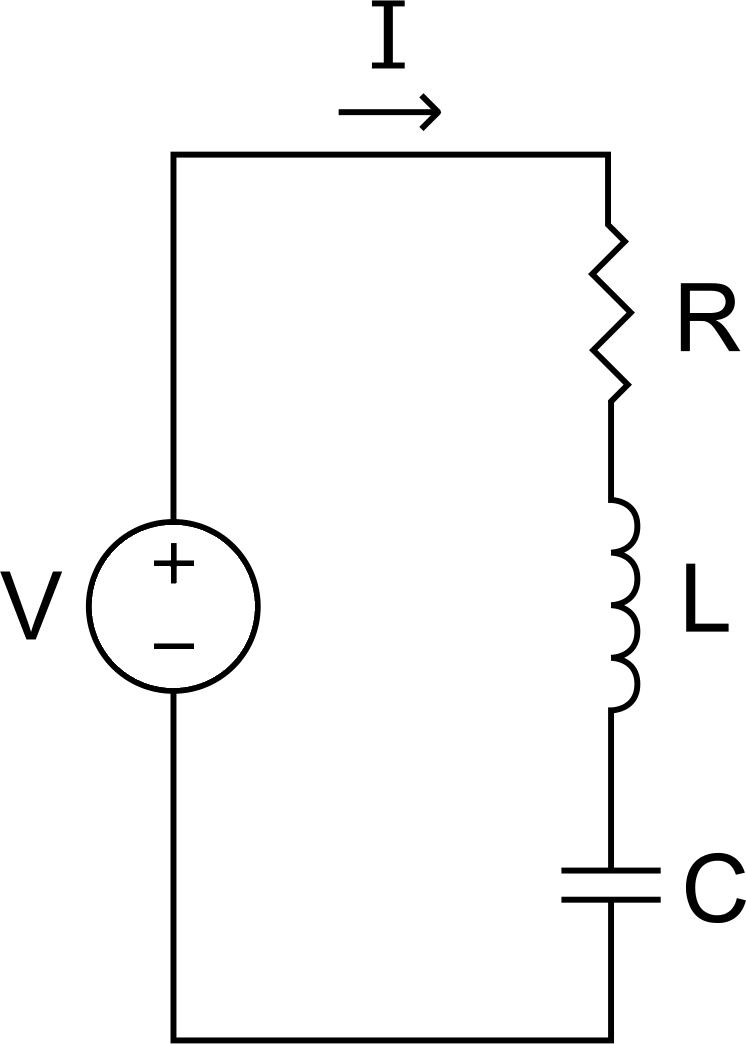
\includegraphics[height=0.34\textwidth]{figures/RLC_series.png} &   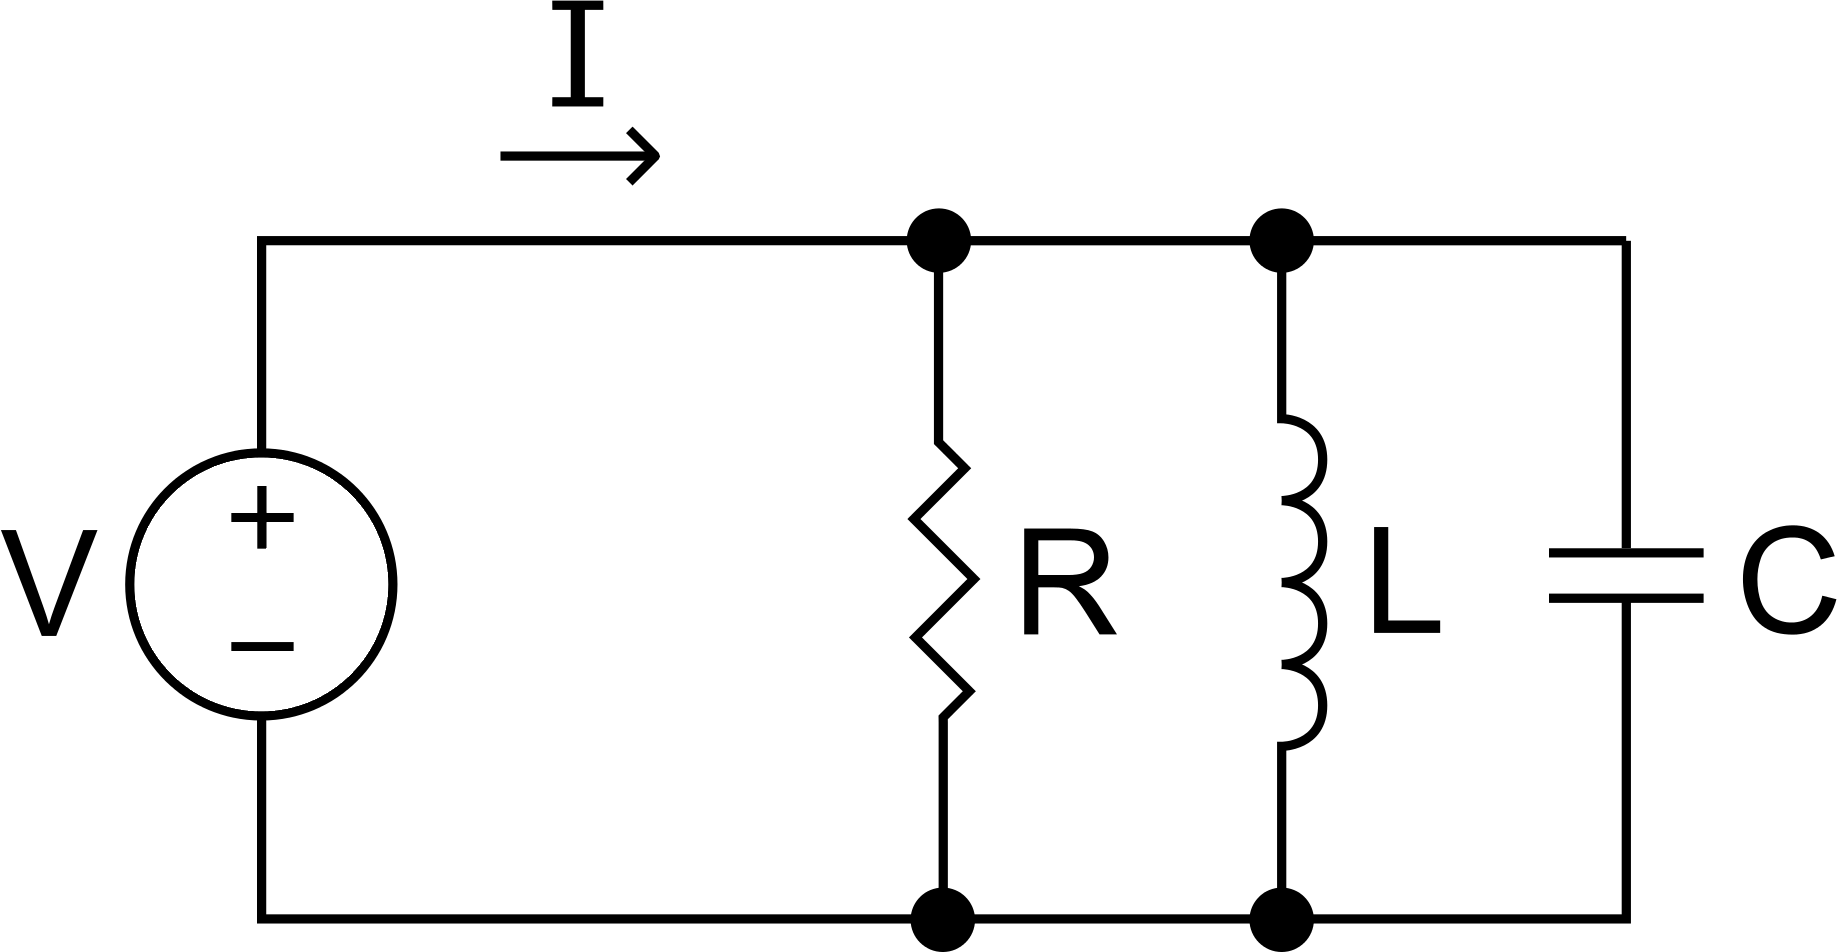
\includegraphics[height=0.30\textwidth]{figures/RLC_parallel.png} \\
(a) Series & (b) Parallerl \\[6pt]
  \centering 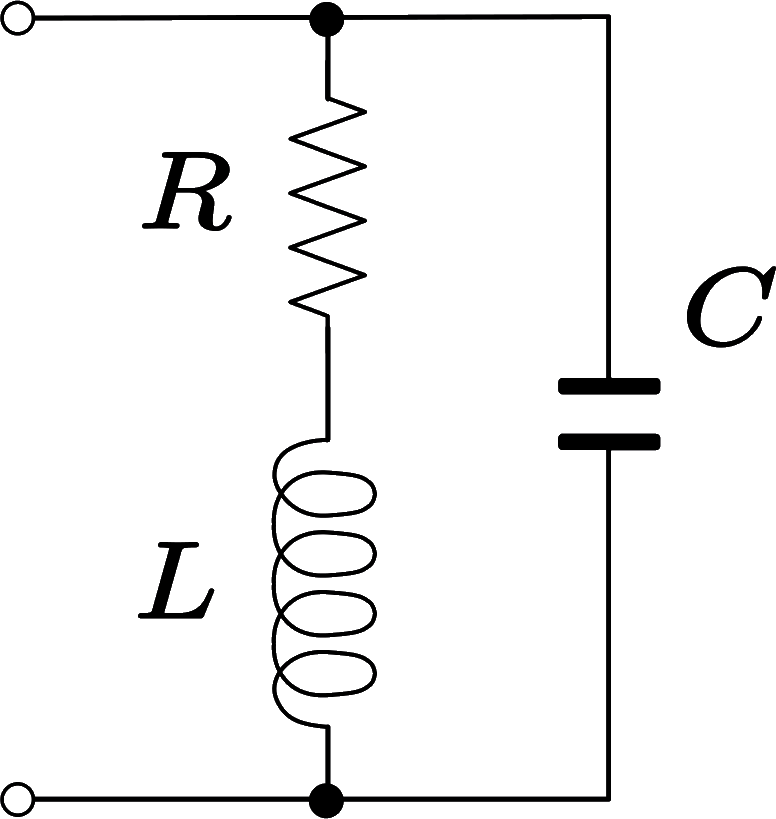
\includegraphics[height=0.35\textwidth]{figures/RL_series_C_parallel.png} &   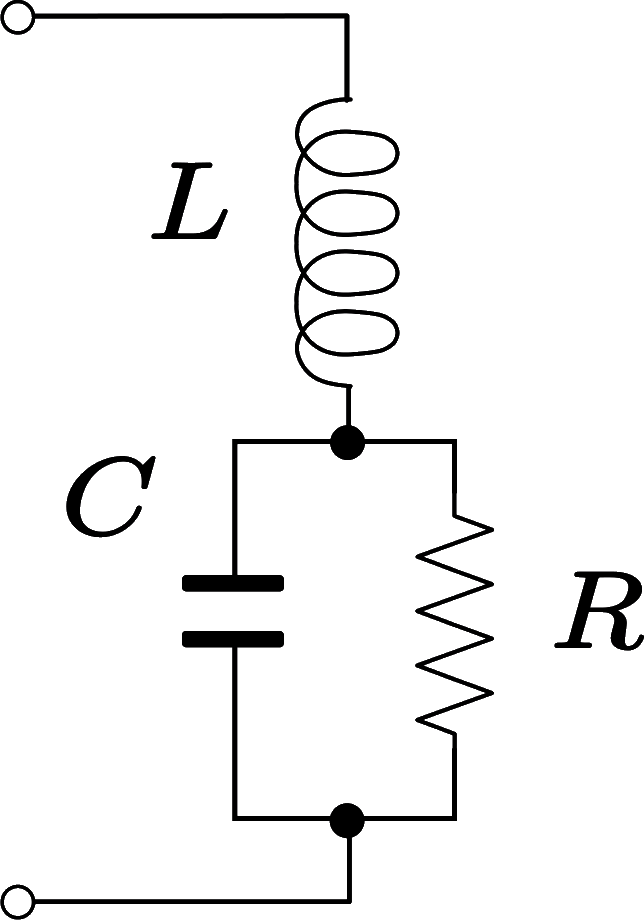
\includegraphics[height=0.35\textwidth]{figures/L_series_RC_parallel.png} \\
(c) third & (d) fourth \\[6pt]
\end{tabular}
\caption{caption}
\end{figure}



\subsection{Pozo de potencial infinito}
\noindent Para la representación usual de este problema se utiliza la en dónde se ubica una partícula de masa m en un espacio limitado por dos barreras de potencial alejadas, una de la otra, con una distancia constante L. Además, se afirma que en el espacio considerado, la partícula de masa m no está sujeta a ninguna fuerza. Esto obliga a una partícula vivir en un intervalo, elegido convencionalmente para ser $x\in [0, a]$. Teniendo en los extremos 0 y a que impiden que la partícula vaya de $x>a$ y $x<0$. El potencial se define de la siguiente manera:.
Este diagrama se denomina escalera cuántica. El nivel de energía más bajo se llama estado fundamental, mientras que el resto se denomina estados excitados.

\subsection{Dependencia del tiempo}
Si una partícula en una caja comienza en una de las funciones propias de energía $\Psi_n(x)$, se multiplica $\Psi_n$ por el factor de ondulación habitual dependiente del tiempo para obtener:
\begin{equation}
    \Psi(x, t)=\Psi_n(x)e^{-iE_nt/\hbar}
\end{equation}
Esto quiere decir que la magnitud de la función de onda permanece sin cambios en cada x, mientras que la fase estará oscilando en el sentido de las agujas del reloj, a una velocidad proporcional a la energía $E_n$
\subsection{Ortogonalidad}
Las autofunciones de energía son ortogonales, en el sentido de que:
\begin{equation}
    \int_{0}^{a} \Psi_m(x)\Psi_n(x)dx=0 \quad m\neq n \label{orthogonal}
\end{equation}
Esta integral se puede ver como un producto punto de dimensión infinita, multiplicando los componentes de $\Psi_m$ y $\Psi_n$ con cada x, para después sumar, para esto, definimos el producto interno de dos funciones de onda undimensionale como:
\begin{equation}
    \langle \Psi_a, \Psi_b \rangle=\int_{-\infty}^{\infty} \Psi_a*(x)\Psi_b(x)dx
\end{equation}
Donde se requiere la conjugación compleja para garantizar el producto interno de cualquier función de onda normalizada, combinando la ecuación \ref{orthogonal} con la condición de normalización, obtenemos:
\begin{equation}
    \int_{0}^{a} \Psi_m(x)\Psi_n(x)dx=\delta_{mn} \label{normalization}
\end{equation}
Donde la $\delta_{mn}$ es una abreviatura de la delta de Kronecker, definido como:
\begin{equation}
    \delta_{mn}=\begin{cases}
1, & \text{if}\quad m=n, \\ 0 & \text{if}\quad m\neq n\end{cases}
\end{equation}
De manera que se puede expresar de forma verbal la ecuación \ref{normalization} como que las funciones propias de la energía son ortonormales.
\subsection{Probabilidad}
Si una partícula en un pozo de potencial infinito comienza con una función propia de energía y se toma la medida de sus posiciones, se podrá saber las probabilidades de los resultados.
La densidad de probabilidad de posición se distribuye en todo el ancho del pozo, y varía sinusoidalmente entre 0 en los nodos y $2/a$ en los antinodas.
Por otro lado, si la partícula comienza en una función de onda arbitraria, si la función es una energía propia de $\Psi_n$, entonces, se obtendra el valor de $E_n$.
Si la función de onda es una mezcla de dos funciones propias de energía, tal como:
\begin{equation}
    \Psi(x)=c_1\Psi_1(x)+c_2\Psi_2(x)
\end{equation}
Entonces, se podran obtener $E_1$ o $E_2$ como resultado, con probabilidades que dependeran de los coeficientes $c_1$ y $c_2$. Es importante mencionar que las probabilidades no pueden ser igual a los coeficientes, ya que estos pueden ser negativos o incluso complejos; las probabilidades son iguales al cuadrado de los módulos de estos coeficientes, $|c_1|^2$ y $|c_2|^2$, respectivamente. Para ver por qué, primero se comprobará la normalización de $\Psi(x)$:
\begin{equation}
    1=\int_{0}^{a}|\Psi(x)|^2dx=\int_{0}^{a}[|c_1|^2\Psi_{1}^{2}+|c_2|^2\Psi_{2}^{2}+(c_1^*c_2+c_2^*c_1)\Psi_1\Psi_2]dx
\end{equation}
integrando los tres términos por separado, encontramos que los dos primeros dan como resultado $|c_1|^2$ y $|c_2|^2$, ya que $\Psi_1$ y $\Psi_2$ están normalizados, mientras que el tercer término integra a cero, ya que $\Psi_1$ y $\Psi_2$ son ortogonales. Por lo tanto, los coeficientes al cuadrado obedecen la relación $|c_1|^2+|c_2|^2=1$, tal como se espera para las probabilidades.
Por lo tanto, según el resultado que se obtienen con el truco de Fourier que menciona el Griffiths, la probabilidad será:
\begin{equation}
    (\text{Probability of}\quad E_n)=|c_n|^2=|\int_{0}^{a}\Psi_n(x)\Psi(x)dx|^2
\end{equation}
Además, la normalización de $\Psi(x)$ implica que la suma de todas estas probabilidades es igual a 1:
\begin{equation}
    \sum_{n=1}^{\infty}|c_n|^2=1
\end{equation}

\subsection{Unidad atómicas}
Las unidades atómicas de Hartree son un sistema de unidades naturales de medición que es especialmente conveniente para los cálculos de física atómica y química computacional. Llevan el nombre del físico Douglas Hartree. Por definición, las siguientes cuatro constantes físicas fundamentales pueden expresarse cada una como el valor numérico 1, multiplicado por una unidad coherente de este sistema:

\begin{itemize}
    \item  Constante de Planck reducida: $\hbar$ , también conocida como la unidad atómica de acción.
\item Carga elemental: $e$, también conocida como la unidad atómica de carga.
\item Radio Bohr: $a_{0}$ también conocida como la unidad atómica de longitud.
\item Mass electrónica: $m_{\text{e}}$, también conocida como la unidad atómica de masa
\end{itemize}

Las unidades atómicas a menudo se abrevian "a.u." o "au", que no deben confundirse con las mismas abreviaturas utilizadas también para unidades astronómicas, unidades arbitrarias y unidades de absorbancia en otros contextos.
%%%%%%%%%%%%%%%%%%%%%%%%%%%%%
%% Numerical methodology
%%%%%%%%%%%%%%%%%%%%%%%%%%%%%
\section{Metodología Numérica}
\subsection{Método de diferencias finitas para problemas lineales}

En el método de diferencias finitas, se utilizan fórmulas de diferencia finita en una malla de puntos igualmente espaciados para  aproximar las derivadas de la ecuación diferencial. En este método, el tamaño de paso h no puede ser muy pequeño ya que existe una estabilidad general de las aproximaciones de la derivada. La forma de la ecuación diferencial de segundo orden con valor a la frontera se encuentra en la ecuación 16.
\begin{equation}
    y''=p(x)y'+q(x)y+r(x),\hspace{10mm}a\leq x\leq b,\hspace{10mm}y(a)=\alpha, y(b)=\beta
\end{equation}
 Para aproximar por medio de cociente de diferencia a $y'$ y $y''$, se debe seleccionar un entero N$\leq$0 y dividimos el intervalo de $[a,b]$ en $(N+1)$ secciones, lo que nos da un tamaño de paso de $h=b-a/N+1$, y los extremos de las secciones se encuentran en los puntos de de malla $x_i=a+ih$ para $i=0,1,...,N+1$.

 Por lo tanto, la ecuación diferencial a aproximar de manera discreta es:
 \begin{equation}
     y''(x_i) = p(x_i)y'(x_i) + q(x_i)y(x_i)+r(x_i)
 \end{equation}
 se expande en el polinomio de Taylor hasta el tercer término alrededor de $x_i$ y evaluado en $x_{i+1}$, tenemos que:
 \begin{equation*}
     y(x_{i+1})= y(x_i) + hy'(x_i)+\frac{h^2}{2}y''(x_i)+\frac{h^3}{6}y'''(x_i) 
 \end{equation*}
 y, al evaluar en $x_{i-1},$ tenemos que:
  \begin{equation*}
     y(x_{i-1})= y(x_i) - hy'(x_i)+\frac{h^2}{2}y''(x_i)-\frac{h^3}{6}y'''(x_i) 
 \end{equation*}
Cuando se suman estas ecuaciones y se resuelve para $y''(x_i)$, tenemos que:
\begin{equation}
    y''(x_i)=\frac{1}{h^2}\left[y(x_{i+1}-2y(x_i)+y(x_{i-1}))\right]
\end{equation}
 La cual recibe el nombre de \textbf{fórmula de diferencia centrada}.
 Por el otro lado, la fórmula de diferencia centrada para $y'(x_i)$ es:
 \begin{equation}
     y'(x_i)=\frac{1}{2h}\left[y(x_{i+1}-x_{i-1})\right]
 \end{equation}
 Utilizando estas dos últimas ecuaciones y reemplazándolas en la ecuación 17, obtenemos la siguiente expresión:

\begin{equation}
    \frac{y(x_{i+1})-2y(x_i)+y(x_{i-1}))}{h^2}=p(x_i)\left[\frac{y(x_{i+1})-y(x_{i-1})}{2h}\right] + q(x_i)y(x_i)+r(x_i)
\end{equation}

De esta manera, se tiene un método de diferencias finitas que nos permite definir un sistema de ecuaciones lineales con $w_0=\alpha$ y $w_{N+1}=\beta$, sustituyendo la expresión $w_i$ por la evaluación de la función $y(x_i)$, se obtiene:

\begin{equation}
    \frac{-w_{i+1}+2w_i-w_{i-1}}{h^2}+p(x_i)\left[\frac{w_{i+1}-w_{i-1}}{2h}\right] + q(x_i)w_i=-r(x_i)
\end{equation}
Para cada $i=1,2,...N.$ Al ordenar términos, se obtiene la siguiente expresión:
\begin{equation*}
    -\left(1+\frac{h}{2}p(x_i)\right)w_{i-1}+(2+h^2q(x_i))w_i-\left(1-\frac{h}{2}p(x_i)\right)w_{i+1}=-h^2r(x_i),
\end{equation*}
Donde podemos observar que los coeficientes de cada $w_i$, $w_{i-1}$ y $w_{i+1}$ se pueden representar en una matriz tridiagonal de tamaño $N\times N$. De esta manera, se representa el sistema como:
\begin{equation}
    \textbf{Aw} = \textbf{b}
\end{equation}
Donde $\textbf{w}=\left[w_1,w_2,...,w_N\right]$;

\begin{equation*}
\textbf{b}=
\begin{pmatrix}
    -h^2r(x_1)+\left(1+\frac{h}{2}p(x_1)\right)w_0 \\
    -h^2r(x_2) \\
    \vdots \\
    -h^2r(x_{N-1}) \\
    -h^2r(x_N)+\left(1+\frac{h}{2}p(x_N)\right)w_{N+1} \\
\end{pmatrix}
\end{equation*}
y,

\begin{equation*}
\textbf{A}=
\begin{pmatrix}
    2+h^2q(x_1) & -1+\frac{h}{2}p(x_1) & 0 & \hdots & 0\\
    -1-\frac{h}{2}p(x_2) & 2+h^2q(x_2) & -1+\frac{h}{2}p(x_1) & \ddots & \vdots  \\
    0 & \ddots & \ddots & \ddots & 0 \\
    \vdots & \ddots & \ddots & \ddots & -1+\frac{h}{2}p(x_{N-1}) \\
    0 & \hdots & 0 & -1-\frac{h}{2}p(x_N) & 2+h^2q(x_N) \\
\end{pmatrix}
\end{equation*}


Es así que se puede desarrollar un algoritmo que implemente la solución de una matriz tridiagonal, por ejemplo, la factorización LU, la cual se puede implementar dentro del algoritmo del método. 
%%%%%%%%%%%%%%%%%%%%%%%%%%%%%
%% Analysis of numerical results
%%%%%%%%%%%%%%%%%%%%%%%%%%%%%
\section{Análisis de resultados numéricos}
Sin embargo, para su análisis es necesario también representar la densidad de probabilidad, es decir el cuadrado de la función de onda, pues esta es un mejor indicador de la probabilidad de encontrar a la partícula en un valor de la posición determinado. Por simple observación, podemos encontrar que en las posiciones de los nodos encontrados de la función de onda existirá la menor probabilidad de encontrar a la partícula. Y, por el contrario, en las posiciones de los antinodos, encontraremos centrados picos, que indican que en estos lugares tenderemos la mayor probabilidad de avistamiento.

Ahondado en lo discutido en el punto anterior, la función de densidad de probabilidad también nos permite calcular cantidades estadísticamente no ables, por medio de unas simples integrales: los primeros dos momentos de la distribución, $\expval{x}$ y $\expval{x^2}$; así como la desviación estándar ($\sigma$). Estos se presentan en la tabla \ref{tab:statexp}, de donde podemos concluir que si bien todas las distribuciones cuentan con medias centradas en el pozo y son simétricas, difieren en que hay una clara tendencia a la dispersión, correlacionada con el nivel energético, como indica el aumento de la desviación standar. Esto ya lo esperábamos pues con el nivel energético aparecen cada vez más picos de probabilidad que se alejan de la media.

\begin{table}[ht]
    \centering
    \resizebox{\textwidth}{!}{
        \begin{tabular}{cccc}
        \toprule[3pt]
Nivel energético & Posición esperada ($a_0$) & $\expval{x^2}$ ($a^2_0$) & Desviación estándar ($a_0$) \\
        \midrule[2pt]
1 & 0.500 & $0.283$ & $0.181$ \\
2 & 0.498 & 0.318 & 0.266    \\
3 & 0.500 & 0.328 & 0.279    \\
4 & 0.498 & 0.328 & 0.283    \\
        \bottomrule[3pt]
        \end{tabular}}
    \caption{Parámetros estadísticos importantes de la función de densidad de probabilidad.}
    \label{tab:statexp}
\end{table}

De manera similar, si restringimos los rangos de integración, es posible encontrar la probabilidad de encontrar al electrón en cierto intervalo del pozo. Cuatro rangos de interés fueron probados y documentados en la tabla \ref{tab:prop}. Primero encontramos que como anteriormente se dijo que la distribución es simétrica con respecto al centro del pozo, la probabilidad de que se encuentre en la primera o segunda mitad de este es la misma. Además, confirmamos el análisis del aumento de dispersión con el nivel energético, pues la probabilidad de encontrar a la partícula en el primer cuarto del pozo aumenta también. Después se investigo la probabilidad de encontrar al electrón en el centro; como habíamos dicho antes esta va alternando de valor con el nivel, pues para los niveles pares se cuenta con un antinodo en el centro del pozo, lo cual hace casi imposible que se encuentre en tal posición. Por último, nos interesó conocer la probabilidad de encontrar al electrón en el centro del pozo y con un radio marcado por la desviación estándar de cada distribución. Encontramos que el mayor valor se encontró en el primer nivel, con una similitud al parámetro de la distribución estándar. Para mayores niveles eso se disminuye ligeramente.

\begin{table}[h!]
    \centering
    \resizebox{\textwidth}{!}{
        \begin{tabular}{ccccc}
        \toprule[3pt]
       \multicolumn{1}{c}{\multirow{2}{*}{Nivel}} & \multicolumn{4}{c}{Probabilidad de encontrar al electrón en:}\\ 
            & Primera mitad & Primer cuarto & [0.45-0.55] & [$(\expval{x}-\sigma)- (\expval{x}+\sigma)$] \\
        \midrule[2pt]
           1     & 0.512 & $9.273\times 10^{-2}$ & $0.208$ & $0.654$\\
           2     & 0.500 & 0.259 & $7.696\times 10^{-3}$ & $0.567$\\
           3     & 0.512 & 0.305 & $0.193$ & $0.469$\\
           4     & 0.500 & 0.250 & $2.867\times 10^{-2}$ & $0.508$\\
        \bottomrule[3pt]
        \end{tabular}}
    \caption{Probabilidad de encontrar a la partícula en cuatro rangos de interés. [0-0.5] $a_0$, [0-0.25] $a_0$, [0.45-0.55] $a_0$ y una bola con radio de la distribución standar centrada en la media.}
    \label{tab:prop}
\end{table}

\subsection{Comparación con solución teórica}
Finalmente, es indispensable comparar nuestra aproximación numérica con la solución analítica de las funciones de onda, para calcular su validez. En la tabla \ref{tab:error} mostramos tres valores del error calculados: el error medio, el error absoluto medio y la raíz del error cuadrático medio. Estos tres valores calculado indican que la aproximación hecha es muy precisa y confiable para el cálculo de las propiedades antes discutidas.

\begin{table}[ht]
    \centering
    \resizebox{\textwidth}{!}{
        \begin{tabular}{cccc}
        \toprule[3pt]
Nivel energético & Error promedio &  Error absoluto promedio & Raíz del erro cuadrático medio\\
        \midrule[2pt]
        \bottomrule[3pt]
        \end{tabular}}
    \caption{Error del calculo experimental comparado con la solución teórica sinusoidal del problema.}
    \label{tab:error}
\end{table}

\subsection{Ortogonalidad del conjunto solución}
Además de las características individuales de las funciones, también nos interesan las cualidades del conjunto, por ejemplo si el conjunto de solución del problema es ortonormal. Recordemos que la normalidad se garantizó en el código, al calcular la integral del cuadrado de las funciones en la totalidad del pozo. Por ello, para el caso de la ortogonalidad, se decidió calcular la \textit{matriz de ortogonalidad} $\mathcal{O}$, cuyas entradas están conformadas por los productos punto de las funciones. Si el resultado de dichas integrales es una matriz que se asemeje a la identidad, entonces es posible afirmar que el conjunto es ortonormal, y esto es justamente lo encontrado en los resultados, eq. \ref{eq:ortm}.

\begin{equation}\label{eq:ortm}\mathcal{O} =\begin{pmatrix}
1.000               &  6.638\times 10^{-3} &  1.229\times 10^{-5} & 2.642\times 10^{-3}\\
6.638\times 10^{-3} &  0.999               & -1.194\times 10^{-2} & 2.636\times 10^{-5}\\
1.229\times 10^{-5} & -1.194\times 10^{-2} &  0.999               & 1.696\times 10^{-2}\\
2.642\times 10^{-3} &  2.636\times 10^{-5} &  1.696\times 10^{-2} & 1.000\\
\end{pmatrix}  \approx \mathcal{I} \end{equation} 


%%%%%%%%%%%%%%%%%%%%%%%%%%%%%
%% Conclusions
%%%%%%%%%%%%%%%%%%%%%%%%%%%%%
\section{Conclusiones}
\noindent Después del análisis de resultados concluimos que el método de diferencias finitas es un método válido y útil para describir el fenómeno de una partícula en el pozo de potencial infinito, pues de los datos se puede apreciar la extraordinaria similitud con la solución analítica. Sin embargo, también hay que reconocer que esta metodología resulta incompleta, pues requerimos del valor de la energía apriori al cálculo de cada función de onda. Por esta razón este método palidece a los utilizados anteriormente para resolver este mismo problema con condiciones iniciales, como el método del disparo.\cite{bobrow1983analisis}



%%%%%%%%%%%%%%%%%%%%%%%%%%%%%
%% References
%%%%%%%%%%%%%%%%%%%%%%%%%%%%%
\newpage\thispagestyle{empty}
\printbibliography\addcontentsline{toc}{section}{References}

%%%%%%%%%%%%%%%%%%%%%%%%%%%%%
%% Appendix (code)
%%%%%%%%%%%%%%%%%%%%%%%%%%%%%
\newpage\thispagestyle{empty}
\appendix
\section{Appendix: Fortran Code}
\begin{code}\begin{lstlisting}[language=fortran,caption={Fortran code that solves the problem of a particle in a one dimentional infinite square well by the fine differences method. It solves for the functions, probability densities, orthogonality matrix, and a few statistically important integrals for the analisys of the first n energy levels. }, label=cd:fortran_gral]

program main
  use, intrinsic :: iso_fortran_env, only: sp=>real32, dp=>real64
  implicit none
  integer,parameter :: n=400, niveles=4
  real(dp),parameter :: x0=0, xf=1, fx0=1, fxf=1
  integer::i,j
  real(dp)::x,h,a(n),b(n),c(n),d(n),l(n),u(n),z(n),w(0:n+1),int_y
  real(dp)::fs(0:n+1,0:niveles),ort(niveles,niveles),dummy,dummy2,sigma

h=(xf-x0)/(n+1)
w(0)=fx0
w(n+1)=fxf
open(101,file="sh_n.dat")
open(100,file="sh.dat")
open(99,file="sh_n2.dat")

     do j=1,niveles
x=x0+h
a(1)=2+h*h*q(j,x) 
b(1)=-1+h*p(x)/2 
d(1)=-h*h*r(x)+(1+h*p(x)/2)*fx0 

!%##for ,nner inner point
do i = 2,n-1
        x=x0+h*i
        a(i)=2+h*h*q(j,x) 
        b(i)=-1+h*p(x)/2 
        c(i)=-1-h*p(x)/2 
        d(i)=-h*h*r(x)
enddo

!##for last inner point
x=xf-h
a(n)=2+h*h*q(j,x) 
c(n)=-1-h*p(x)/2 
d(n)=-h*h*r(x)+(1-h*p(x)/2)*fxf 
!##vectors a,b,c,d are populated

!#Solving the matrix
l(1)=a(1)
u(1)=b(1)/a(1)
z(1)=d(1)/l(1)

do i = 2,n-1
        l(i)=a(i)-c(i)*u(i-1)
        u(i)=b(i)/l(i)
        z(i)=(d(i)-c(i)*z(i-1))/l(i)
enddo

l(n)=a(n)-c(n)*u(n-1)
z(n)=(d(n)-c(n)*z(n-1))/l(n)

do i = 1,n
        w(i)=z(i)-fx0
enddo

do i = n-1,1,-1
        w(i)=z(i)-u(i)*w(i+1)
enddo

do i=0,n+1
        if (j==1) then
                fs(i,0)= x0+i*h
        endif
        write(100,*) fs(i,0), w(i)
enddo
write(100,*)  " "
int_y=simple_integral(h,w)
int_y=int_y

do i=0,n+1
        fs(i,j)=w(i)/sqrt(int_y)
        write(101,*) fs(i,0), fs(i,j)
        write(99,*) fs(i,0), fs(i,j)*fs(i,j)
enddo
write(101,*)  " "
write(99,*)  " "

        enddo
close(99)
close(100)
close(101)

do i=1,niveles
        do j=1,niveles
                ort(i,j)=double_integral(h,fs(:,i),fs(:,j))
        enddo
enddo

open(102,file="sh.ortm")
do i=1,niveles
        write(102,*) ort(:,i)
enddo
close(102)

open(103,file="sh.stat")
do i=1,niveles
        dummy=expx(h,fs(:,0),fs(:,i))
        dummy2=expx2(h,fs(:,0),fs(:,i))
        sigma=sqrt(dummy2-dummy*dummy)
        write(103,*) "       <x> for level",i," is ", dummy
        write(103,*) "      <x2> for level",i," is ", dummy2
        write(103,*) "<x2>-<x>^2 for level",i," is ", dummy2-dummy*dummy
        write(103,*) "        SD for level",i," is ", sigma
        write(103,*) "Probability to to find electron between x+sigma and x-sigma"
        write(103,*)  prob(h,fs(:,0),fs(:,i), dummy-sigma , dummy+sigma)
        write(103,*) "Probability to to find electron between 0.45 and 0.55"
        write(103,*)  prob(h,fs(:,0),fs(:,i), 0.45D0, 0.55D0)
        write(103,*) "Probability to to find electron on the left side"
        write(103,*)  prob(h,fs(:,0),fs(:,i), 0D0, 0.5D0)
        write(103,*) "Probability to to find electron on the first quarter"
        write(103,*)  prob(h,fs(:,0),fs(:,i), 0D0, 0.25D0)
        write(103,*) " "
enddo
close(103)


contains
real(dp) function p(r) result(f)
  implicit none
  real(dp), intent(in) :: r
    f = 0D0
end function p

real(dp) function q(well_n, r) result(E)
  implicit none
  real(dp), intent(in) :: r
  integer, intent(in) :: well_n
  real(dp), parameter:: m=1D0,  pi=3.14159265
    E =-(well_n*pi*well_n*pi)
end function q

real(dp) function r(x) result(f)
  implicit none
  real(dp), intent(in) :: x
    f = 0D0
end function r

real(dp) function simple_integral(h,y) result(f)
  real(dp), intent(in) :: h, y(0:)
  integer ::i
    f=y(0)*y(0)
    do i=1, (size(y)-1)/2
         f=f+4*y(2*i-1)*y(2*i-1)
    enddo
    do i=2, (size(y)-1)/2-1
         f=f+2*y(2*i)*y(2*i)
    enddo
    f=f+y(size(y)-1)*y(size(y)-1)
    f=f*h/3
end function simple_integral

real(dp) function double_integral(h,y,w) result(f)
  real(dp), intent(in) :: h, y(0:), w(0:)
  integer ::i
    f=w(0)*y(0)
    do i=1, (size(y)-1)/2
         f=f+4*w(2*i-1)*y(2*i-1)
    enddo
    do i=2, (size(y)-1)/2-1
         f=f+2*w(2*i)*y(2*i)
    enddo
    f=f+w(size(y)-1)*y(size(y)-1)
    f=f*h/3
end function double_integral

real(dp) function prob(h,x, w,a,b) result(f)
  real(dp), intent(in) :: h, x(0:), w(0:), a, b
  integer :: xa(1), xb(1)
  integer ::i , ia , ib
    xa=minloc(abs(x-a))
    xb=minloc(abs(x-b))
    ia=xa(1)
    ib=xb(1)
    if (MOD(ib-ia,2)==0) then
        f=w(ia)*w(ia)
        do i=ia+1, ib-1, 2
             f=f+4*w(i)*w(i)
        enddo
        do i=ia+2, ib-1, 2
             f=f+2*w(i)*w(i)
        enddo
        f=f+w(ib)*w(ib)
        f=f*h/3
    else 
        ib=ib+1
        f=w(ia)*w(ia)
        do i=ia+1, ib-1, 2
             f=f+4*w(i)*w(i)
        enddo
        do i=ia+2, ib-1, 2
             f=f+2*w(i)*w(i)
        enddo
        f=f+w(ib)*w(ib)
        f=f*h/3
    endif
end function 

real(dp) function expx(h,x,w) result(f)
  real(dp), intent(in) :: h, x(0:), w(0:)
  integer ::i
    f=x(0)*w(0)*w(0)
    do i=1, (size(w)-1)/2
        f=f+4*x(2*i-1)*w(2*i-1)*w(2*i-1)
    enddo
    do i=2, (size(w)-1)/2-1
        f=f+2*w(2*i)*w(2*i)*x(2*i)
    enddo
    f=f+x(size(x)-1)*w(size(w)-1)*w(size(w)-1)
    f=f*h/3
end function 
        
real(dp) function expx2(h,x,w) result(f)
  real(dp), intent(in) :: h, x(0:), w(0:)
  integer ::i
    f=x(0)*x(0)*w(0)*w(0)
    do i=1, (size(w)-1)/2
        f=f+4*x(2*i-1)*x(2*i-1)*w(2*i-1)*w(2*i-1)
    enddo
    do i=2, (size(w)-1)/2-1
        f=f+2*w(2*i)*w(2*i)*x(2*i)*x(2*i)
    enddo
    f=f+x(size(x)-1)*x(size(x)-1)*w(size(w)-1)*w(size(w)-1)
    f=f*h/3
end function 

end program



\end{lstlisting}
\end{code}

\end{document}
